\SourcePage{698}{703}
\section{Low-energy theorem for photon scattering by a hadron}

At low frequencies, the cross section for photon scattering by any stationary charged particle approaches the classical value given by the Thomson formula. This limit corresponds to an amplitude independent of the photon frequency $\omega$; denote it by $M_{fi}^{(0)}$. It turns out, however, that in photon scattering (as in the bremsstrahlung discussed in the preceding section), not only this leading term but also the next term in the expansion of the amplitude in powers of $\omega$ is independent of the details of the hadron's electromagnetic structure:
\begin{equation}
M_{fi}=M_{fi}^{(0)}+M_{fi}^{(1)},
\tag{141.1}
\end{equation}
where $M^{(1)}\sim\omega$ (F.~E.~Low, 1954; M.~Gell-Mann, M.~L.~Goldberger, 1954).

The process is represented by three types of diagram:
\begin{equation}
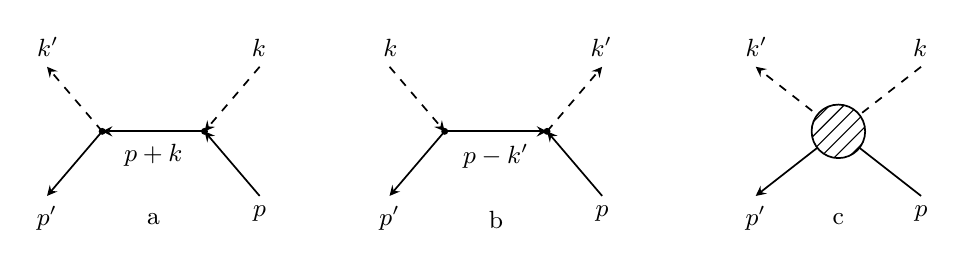
\begin{tikzpicture}[baseline=-.45ex,x=1cm,y=1cm,>=stealth,line width=.62pt,font=\small]
  % (a): s-channel pole graph
  \begin{scope}[xshift=-4.35cm]
    \coordinate (vl) at (-.65,0);
    \coordinate (vr) at (.65,0);
    \draw[->] (vl)--(-1.35,-.82);
    \draw[dashed,->] (vl)--(-1.35,.82);
    \draw[->] (vr)--(vl);
    \draw[->] (1.35,-.82)--(vr);
    \draw[dashed,->] (1.35,.82)--(vr);
    \fill (vl) circle (1.25pt);
    \fill (vr) circle (1.25pt);
    \node[above] at (-1.34,.82) {$k'$};
    \node[below] at (-1.35,-.82) {$p'$};
    \node[above] at (1.34,.82) {$k$};
    \node[below] at (1.35,-.82) {$p$};
    \node[below] at (0,-.03) {$p+k$};
    \node at (0,-1.12) {a};
  \end{scope}
  % (b): u-channel pole graph
  \begin{scope}
    \coordinate (vl) at (-.65,0);
    \coordinate (vr) at (.65,0);
    \draw[->] (vl)--(-1.35,-.82);
    \draw[dashed,->] (-1.35,.82)--(vl);
    \draw[->] (vl)--(vr);
    \draw[->] (1.35,-.82)--(vr);
    \draw[dashed,->] (vr)--(1.35,.82);
    \fill (vl) circle (1.25pt);
    \fill (vr) circle (1.25pt);
    \node[above] at (-1.34,.82) {$k$};
    \node[below] at (-1.35,-.82) {$p'$};
    \node[above] at (1.34,.82) {$k'$};
    \node[below] at (1.35,-.82) {$p$};
    \node[below] at (0,-.03) {$p-k'$};
    \node at (0,-1.12) {b};
  \end{scope}
  % (c): regular graph
  \begin{scope}[xshift=4.35cm]
    \coordinate (v) at (0,0);
    \draw[->] (v)--(-1.05,-.82);
    \draw[dashed,->] (v)--(-1.05,.82);
    \draw[->] (1.05,-.82)--(v);
    \draw[dashed,->] (1.05,.82)--(v);
    \fill[white] (v) circle (.34);
    \begin{scope}
      \clip (v) circle (.34);
      \foreach \d in {-1.0,-.82,...,1.0} {
        \draw[thin] (-.55,\d-.55)--(.55,\d+.55);
      }
    \end{scope}
    \draw (v) circle (.34);
    \node[above] at (-1.04,.82) {$k'$};
    \node[below] at (-1.05,-.82) {$p'$};
    \node[above] at (1.04,.82) {$k$};
    \node[below] at (1.05,-.82) {$p$};
    \node at (0,-1.12) {c};
  \end{scope}
\end{tikzpicture}
\tag{141.2}
\end{equation}
The first two again contain a one-particle intermediate state and therefore have a pole singularity.

The reasoning and the essential features of the calculation are the same as in~\S~140. In fact, it suffices to calculate only the contribution of the pole parts of diagrams~(141.2a--b), with their electromagnetic vertices expressed through the static form factors (the charge $Ze$ and anomalous magnetic moment $\mu_{\text{an}}$).

\SourcePage{699}{704}
Unlike the bremsstrahlung case, however, the corrections to the Compton-scattering cross section that concern us here exist only for particles with spin. In bremsstrahlung, besides the spin-dependent corrections, there are corrections associated with the energy dependence of the amplitude of the ``elastic'' process. Here its role is played by the form factors, which reduce to constants on the ``physical legs'' and have no energy dependence. Thus, for photon scattering the corrections arise solely from the magnetic moment, which spinless particles do not possess. We shall consider below the scattering of a photon by a spin-$1/2$ hadron.

Let $M_{fi}$ now mean the pole-diagram contribution to the scattering amplitude. We then have (cf.~(86.3), (86.4))
\begin{equation}
M_{fi}=-4\pi(Ze)^2e_\mu^{\prime *}e_\nu(\bar u'Q^{\mu\nu}u),
\tag{141.3}
\end{equation}
where
\begin{equation}
\begin{aligned}
Q^{\mu\nu}={}&(\gamma^\mu+S'^{\mu})
\frac{\gamma p+\gamma k+M}{s-M^2}(\gamma^\nu-S^\nu)+{}\\
&+(\gamma^\nu-S^\nu)
\frac{\gamma p-\gamma k'+M}{u-M^2}(\gamma^\mu+S'^{\mu}),
\end{aligned}
\tag{141.4}
\end{equation}
\[
s=(p+k)^2=(p'+k')^2,\qquad
u=(p-k')^2=(p'-k)^2
\]
and, for brevity, the notation
\begin{equation}
\mu_{\text{an}}\sigma^{\mu\lambda}k_\lambda=ZeS^\mu,
\qquad
\mu_{\text{an}}\sigma^{\mu\lambda}k'_\lambda=ZeS'^{\mu}.
\tag{141.5}
\end{equation}
has been introduced. By moving the operators $\gamma p+M$ and using the equations
\[
\bar u'(\gamma p'-M)=(\gamma p-M)u=0,
\]
expression~(141.4) may be transformed into
\begin{equation}
\begin{aligned}
Q^{\mu\nu}={}&\left[(\gamma^\mu+S'^{\mu})
\frac{(\gamma k)\gamma^\nu+2p^\nu}{2(pk)}
+\frac{\gamma^\nu(\gamma k)-2p'^\nu}{2(p'k)}
(\gamma^\mu+S'^{\mu})\right]-{}\\
&-\left[\frac{\gamma^\mu(\gamma k')+2p'^\mu}{2(p'k')}S^\nu
+S^\nu\frac{\gamma^\mu(\gamma k')-2p^\mu}{2(pk')}\right]-{}\\
&-\left[S'^{\mu}\frac{\gamma p+\gamma k+M}{2(pk)}S^\nu
-S^\nu\frac{\gamma p-\gamma k'+M}{2(pk')}S'^{\mu}\right].
\end{aligned}
\tag{141.6}
\end{equation}
Written in this form (or in the analogous form with $k$ and $k'$ interchanged), the gauge invariance of expression~(141.3) is manifest; its conditions are
\begin{equation}
k'_\mu(\bar u'Q^{\mu\nu}u)=(\bar u'Q^{\mu\nu}u)k_\nu=0
\tag{141.7}
\end{equation}
(in checking these relations, recall that $(\gamma k)(\gamma k)=0$ and $kS=k'S'=0$).

\SourcePage{700}{705}
Since the pole part of the scattering amplitude is therefore gauge-invariant by itself, the regular part of the amplitude, which also includes the contribution from diagram~(141.2c), must likewise be gauge-invariant separately. It follows in turn that the expansion of this part in powers of $k$ and $k'$ must begin with quadratic terms (compare the analogous observation concerning condition~(127.5)). In other words, the regular part of the amplitude contains only terms starting at order $\omega\omega'\sim\omega^2$ and hence contributes nothing to the terms proportional to $\omega^0$ and $\omega^1$ that are of interest here. All such terms are consequently contained in expression~(141.3).

For their explicit calculation, choose the laboratory frame in which the initial hadron is at rest. For the photons choose a three-dimensionally transverse gauge, in which $e_0=e'_0=0$. Then $(pe)=0$ and $(p'e'^{*})\sim|\mathbf p'|\sim\omega$. It follows from~(141.6) that the first terms in the expansion of $M_{fi}$ are proportional to $\omega^0$, whereas the terms containing $\mu_{\text{an}}$ contribute only at order $\omega^1$.

To the required accuracy, the wave amplitudes of the initial and final hadrons in the laboratory frame are
\[
u=\sqrt{2M}\begin{pmatrix}w\\0\end{pmatrix},\qquad
\bar u'=\sqrt{2M}\left(w'^{*},-\frac{w'^{*}}{2M}(\mathbf k-\mathbf k')\boldsymbol{\sigma}\right),
\]
where $w$ and $w'$ are 3-spinors.

Direct calculation gives
\begin{equation}
M_{fi}^{(0)}=-8\pi(Ze)^2(\mathbf e'^{*}\mathbf e)(w'^{*}w),
\tag{141.8}
\end{equation}
\begin{equation}
\begin{aligned}
M_{fi}^{(1)}={}&-16\pi iM\mu_{\text{an}}^2\omega
(w'^{*}\boldsymbol{\sigma}w)
(\mathbf n'\times\mathbf e'^{*})(\mathbf n\times\mathbf e)-{}\\
&-4\pi iZe\mu_{\text{an}}\omega(w'^{*}\boldsymbol{\sigma}w)
\left\{\mathbf n\bigl((\mathbf n\times\mathbf e)\mathbf e'^{*}\bigr)
+(\mathbf n\times\mathbf e)(\mathbf n\mathbf e'^{*})-{}\right.\\
&\hspace{10em}\left.{}-\mathbf n'\bigl((\mathbf n'\times\mathbf e'^{*})\mathbf e\bigr)
-(\mathbf n'\times\mathbf e'^{*})(\mathbf n\mathbf e)
-2(\mathbf e'^{*}\times\mathbf e)\right\},
\end{aligned}
\tag{141.9}
\end{equation}
where $\mathbf n=\mathbf k/\omega$ and $\mathbf n'=\mathbf k'/\omega'$.

The scattering cross section is
\begin{equation}
d\sigma=\frac{1}{64\pi^2}|M_{fi}|^2\frac{\omega'^2}{M^2\omega^2}\,do'
\tag{141.10}
\end{equation}
(see~(64.19)). For scattering by a charged particle, both $M_{fi}^{(1)}$ and $M_{fi}^{(0)}$ are nonzero. At the adopted accuracy, the terms $|M_{fi}^{(0)}|^2$ and $\operatorname{Re}(M_{fi}^{(0)}M_{fi}^{(1)*})$ may therefore be retained in the square $|M_{fi}|^2$. The former gives the Thomson cross section. The latter, however, vanishes

\SourcePage{701}{706}
after averaging over photon and hadron polarizations. Thus, in scattering by a charged hadron, the corrections under consideration appear only in polarization effects.

For scattering by an electrically neutral hadron, on the other hand, $M_{fi}^{(0)}=0$, and the cross section is determined by $|M_{fi}^{(1)}|^2$. After averaging over the initial-particle polarizations and summing over those of the final particles, it is (in conventional units)
\begin{equation}
d\sigma=\frac{2\mu^4\omega^2}{\hbar^2c^4}(2+\sin^2\vartheta)\,do',
\tag{141.11}
\end{equation}
where $\vartheta$ is the photon scattering angle and the anomalous magnetic moment is the same as the total moment $\mu$. In its angular dependence, this cross section corresponds to antisymmetric scattering (see problem~2 in~\S~60).
